\documentclass[11pt]{article}
\usepackage[utf8]{inputenc}
\usepackage[T1]{fontenc}
\usepackage[margin = 2cm]{geometry}

\usepackage{palatino}
\usepackage{amsmath}
\usepackage{graphicx}
\usepackage{listings}
\usepackage{mathpazo}
\usepackage{hyperref}
\usepackage{courier}
\usepackage{subfigure}

\lstset{basicstyle=\normalsize\ttfamily, breaklines=true}

\author{Samuele Bosi, Marco Ferrè, Philip Michael Grasselli, Simone Mariani}
\title{\textbf{CMLS Homework 2 – Subtractive Synthesis}}
\date{\today}

\begin{document}
\maketitle
\tableofcontents

\section{Introduction}
In this homework, our main task was to implement a synthesizer based on \textbf{subtractive synthesis}: when a tymbrically rich sound (usually referring to the quantity of harmonics) is involved into this procedure, you obtain an altered one, thanks to filters which attenuate defined partials. \\
In fact, this routine is based on two components to muster up:
\begin{itemize}
\item a waveform generator;
\item a filter.
\end{itemize}
A GUI (Graphic User Interface) is also included, in order to both respect the request of the homework, and to have a more practical and clearer experience in understanding subtracting synthesis.\\
To be more practical, we also included a short music track as a demo, in which all sounds are generated by our synthesizer, except for the drums.

\section{The Synthesizer}
The following is a concise guideline on the development of the synthesizer. For a complete reference, we remind to its repository: \url{https://github.com/marcoferre/CMLS-HW2}.

\subsection{GUI}
\begin{figure}
\centering
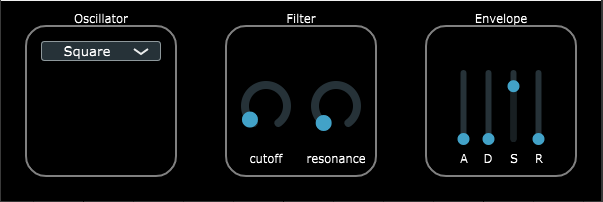
\includegraphics[width=0.5\textwidth]{GUI.png}
\label{fig:GUI}
\caption{A screenshot of the Graphical User Interface}
\end{figure}
Our plug-in, in a essential fashion, sticks to a classic sound chain of a synthesizer based on subtractive synthesis. In further detail, the visible and manageable components are thus represented in Figure \ref{fig:GUI}:
\begin{itemize}
\item an \textbf{oscillator} with three different kinds of waveform available (sine wave, saw-tooth, square wave);
\item a low-pass resonant IIR (Infinite Impulse Response) \textbf{filter};
\item an ADSR (Attack, Decay, Sustain, Release) \textbf{envelope generator} for the output signal.
\end{itemize}

\subsection{The Oscillator}
To develop the oscillator section, the \texttt{maximilian} library is the easiest and most powerful way to implement multi-voice oscillator in the JUCE environment. In particular, our oscillator involves the presence of three different wave forms (sine wave, saw-tooth, square-wave), with an up-to-five voices overlap, so that this produces polyphonic sound. Thus, there's the chance to produce  either \textit{Pad} or \textit{Lead} sounds.

\subsection{The Filter}
We focused on using a IIR filter, and this is fully implemented into JUCE in the class DSP in the following way:

\begin{lstlisting}
dsp::IIR::Coefficients<float>::makeLowPass (double sampleRate, NumericType frequency, NumericType Q)
\end{lstlisting}

The \texttt{makeLowPass} method, in particular, returns a IIR filter with the coefficients adapted to create a \textbf{resonant low-pass filter}. In the GUI, you have its control through the frequency and resonance knobs.\\
The choice of using a IIR filter, instead of a FIR one, is for is very light computational cost, and to take advantage of the instabilities that emerge at high resonance values.

\subsection{The Envelope Generator}
By using the same \texttt{maximilian} library mentioned previously, we added a standard envelope generator based on the \textbf{ADSR procedure}, and applied on the volume level at the output, in order to render the sound timbre more pleasantly listenable.

\section{Linking GUI and Processor}
The links between the GUI and the processor were implemented by applying the class \texttt{ValueTree}. Moreover, this class lets the GUI parameters be exposed to any possible DAW, to external controllers or automation.

\section{Conclusions}

The final result, built as a VST3 and tested in a DAW (Reaper), allows you to set up and appreciate a catchier and more useful sound. Please note that there are means of overcoming the lack of harmonic parts due to the absence of an envelope, such as considering external automation solutions, thanks to its explicit parameters.\\
As measured by an oscilloscope, the output signal shows up a pretty accurate waveform: the instability given by the IIR filter is appreciated whilst high values of resonance are contemplated, and with the typical oscillation close to the jump points, as shown in Figure \ref{fig:waves}.

\begin{figure}
\centering
\subfigure[A saw-tooth wave]{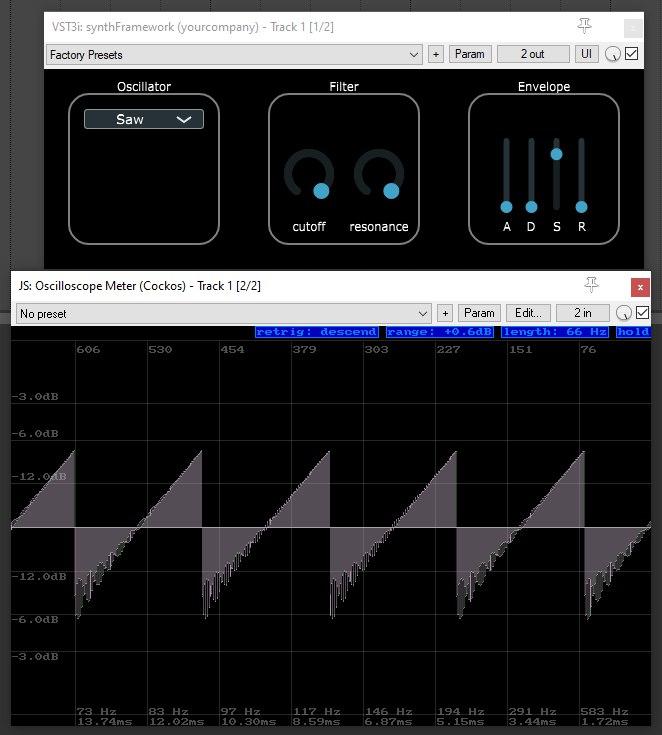
\includegraphics[width=0.4\textwidth]{Sawtooth.jpeg}}
\subfigure[A square wave]{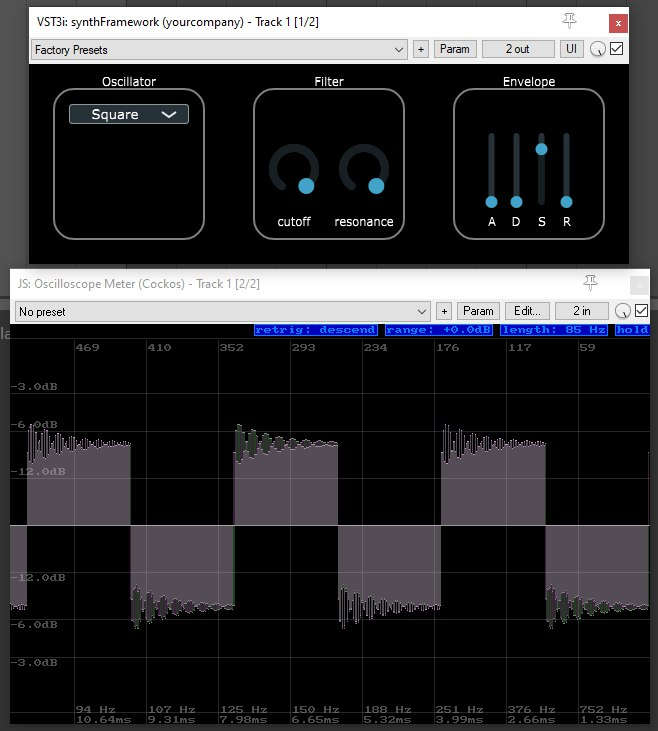
\includegraphics[width=0.4\textwidth]{Square.jpeg}}
\label{fig:waves}
\caption{Effect of the maximum resonance values seen on the oscilloscope, which clearly highlights the oscillation close to the jump points.}
\end{figure}

\end{document}
